% Auto-generated figure snippets for the cross-species BCAP manuscript.
% Each figure's data is traceable to a sentence in inputs/experimental_log.md.

\begin{figure}[htbp]
\centering

\includegraphics[width=0.95\textwidth]{figures/fig1_pipeline.pdf}
\caption{Schematic of the brain structure based cross-species age prediction
pipeline. Structural and diffusion MRI from 370 humans (8--14 years) and 181
macaques (2--4 years) yield 260 per-subject features (92 GMV regions plus FA,
MD, AD, RD over 42 white-matter tracts). Pearson-correlation feature selection
($p < 0.01$) and repeated-iteration stability screening feed four prediction
models trained with 10-fold cross-validation. The models produce within-species
and cross-species age estimates that are combined into the brain cross-species
age gap (BCAP) percentile-rank index.}
\label{fig:pipeline}
\end{figure}

\begin{figure}[htbp]
\centering
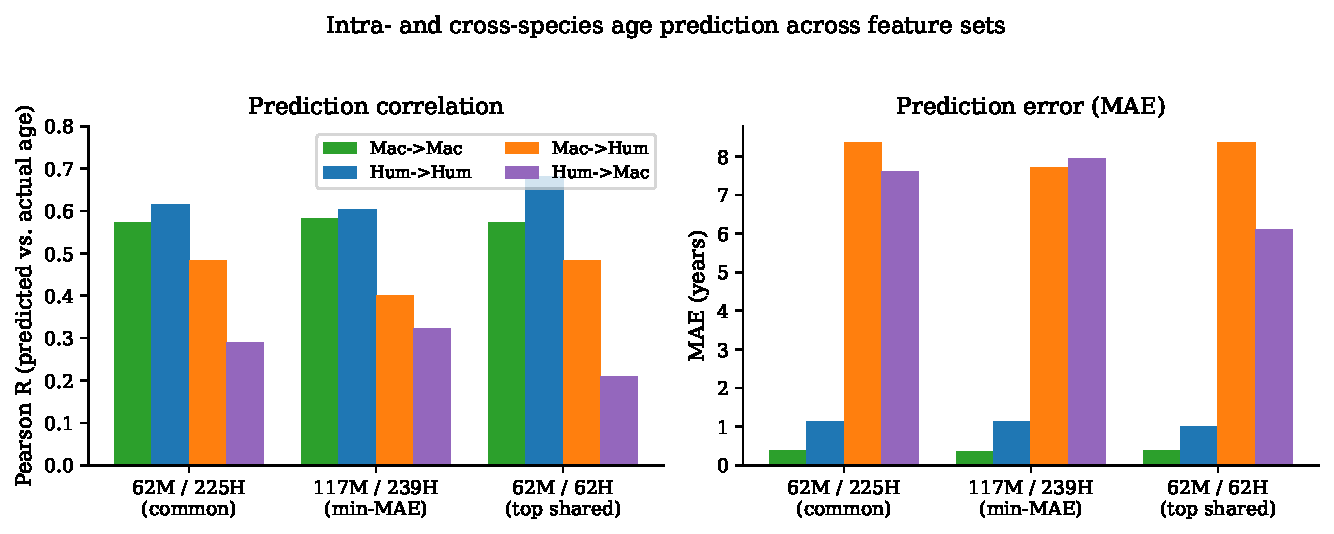
\includegraphics[width=0.95\textwidth]{figures/fig2_prediction_performance.pdf}
\caption{Within- and cross-species age prediction across three feature-set
choices. Left: Pearson correlation $R$ between predicted and actual age.
Right: mean absolute error (MAE, years). Macaque-trained models consistently
predict human age more accurately (Mac$\rightarrow$Hum) than human-trained
models predict macaque age (Hum$\rightarrow$Mac), across all three feature
sets. Values: common-features (62/225): $R_{\text{Mac}\to\text{Mac}}=0.5729$,
$R_{\text{Hum}\to\text{Hum}}=0.6153$, $R_{\text{Mac}\to\text{Hum}}=0.4823$,
$R_{\text{Hum}\to\text{Mac}}=0.2898$; min-MAE (117/239):
$R = 0.5825/0.6039/0.4018/0.3223$; top-62 shared:
$R = 0.5729/0.6818/0.4822/0.2094$.}
\label{fig:prediction_performance}
\end{figure}

\begin{figure}[htbp]
\centering
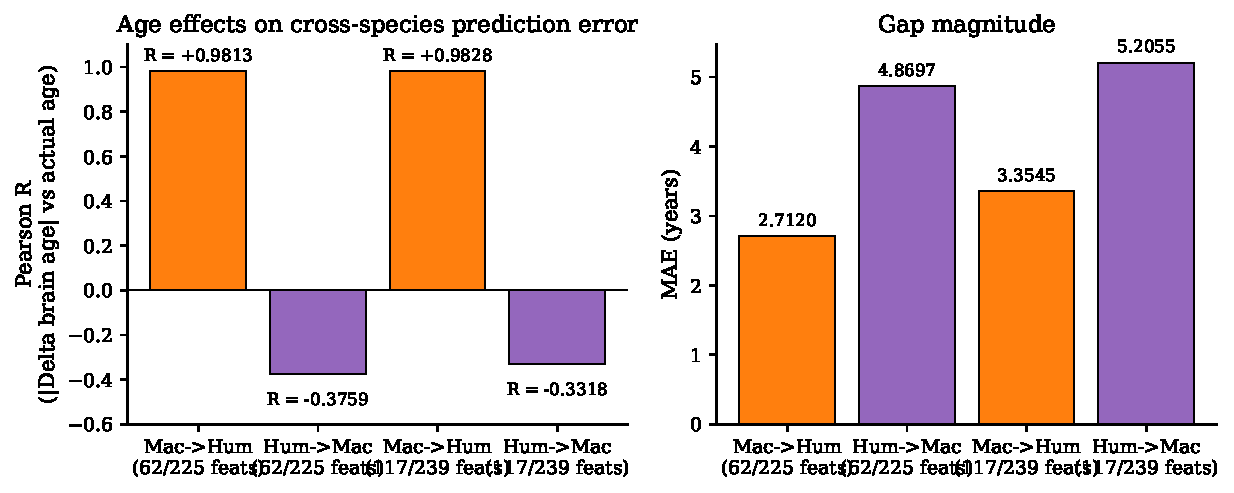
\includegraphics[width=0.9\textwidth]{figures/fig3_age_gap.pdf}
\caption{Relationship between $|\Delta\text{brain age}|$ and actual age in
each species under two feature-selection regimes. Human $|\Delta\text{brain
age}|$ grows with actual age (Mac$\rightarrow$Hum: $R = 0.9813$, $P < 0.001$,
MAE = 2.7120 years; replication at 117/239 feats: $R = 0.9828$, $P = 0.001$,
MAE = 3.3545), while macaque $|\Delta\text{brain age}|$ decreases with actual
age (Hum$\rightarrow$Mac: $R = -0.3759$, $P < 0.001$, MAE = 4.8697;
replication: $R = -0.3318$, $P < 0.001$, MAE = 5.2055). Dashed zero line
separates positive from negative age dependence.}
\label{fig:age_gap}
\end{figure}

\begin{figure}[htbp]
\centering
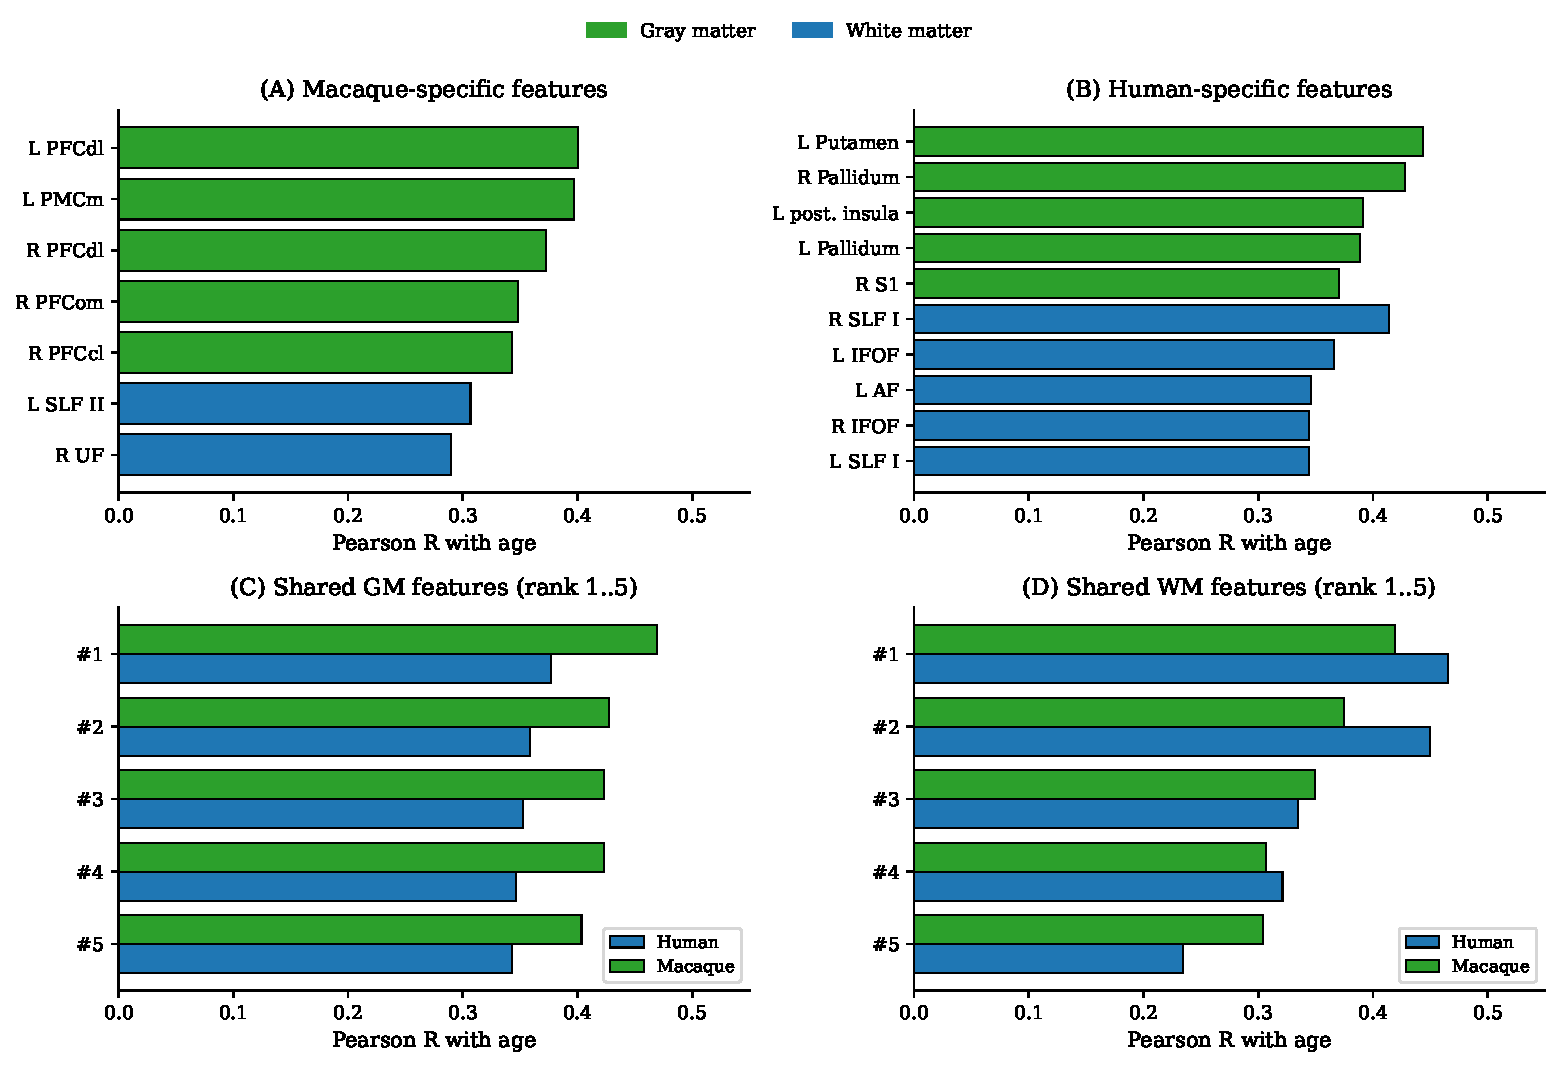
\includegraphics[width=0.95\textwidth]{figures/fig4_features.pdf}
\caption{Top features by Pearson correlation with age.
(A) Macaque-specific: gray-matter (green) in prefrontal and motor regions,
white-matter (blue) in left SLF II and right UF.
(B) Human-specific: gray-matter in basal ganglia, insula, and sensory cortex,
white-matter concentrated in language-related tracts (SLF I, IFOF, AF).
(C) Shared gray-matter features in humans (blue) vs macaques (green), ranked
1--5.
(D) Shared white-matter features in humans vs macaques, ranked 1--5; the
corticospinal tract dominates both species.}
\label{fig:features}
\end{figure}

\begin{figure}[htbp]
\centering
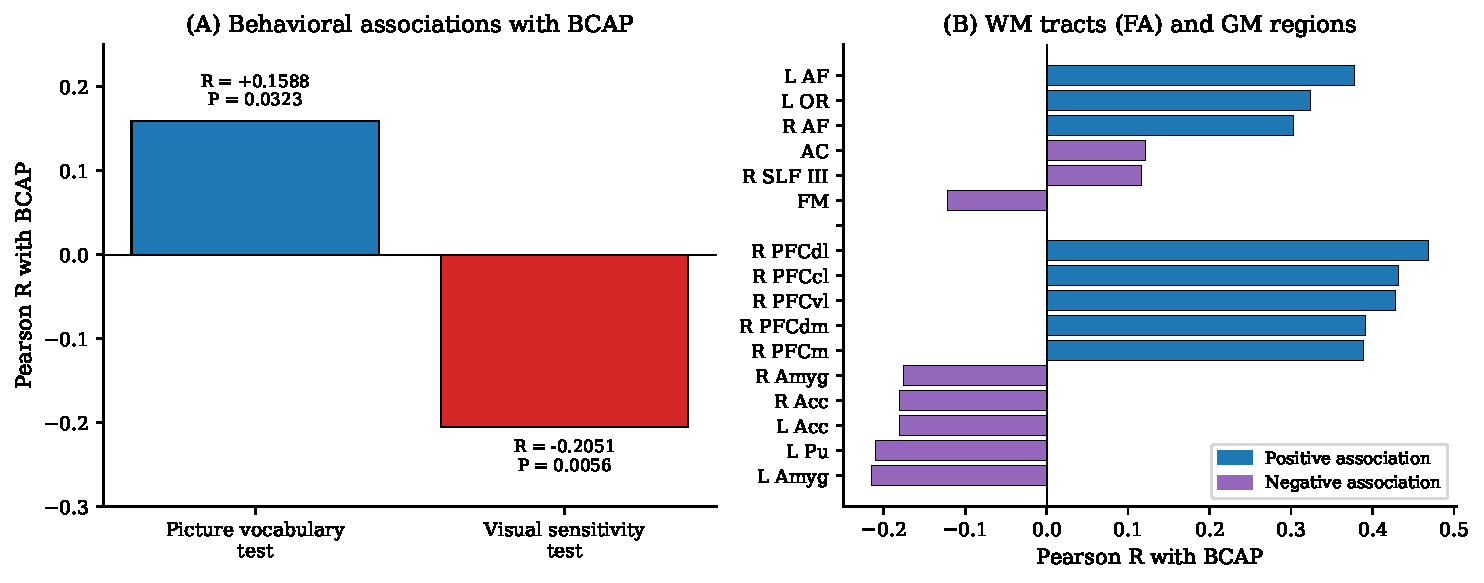
\includegraphics[width=0.95\textwidth]{figures/fig5_bcap.pdf}
\caption{BCAP associations.
(A) Behavioral phenotypes: picture vocabulary test ($R = 0.1588$, $P = 0.0323$)
and visual sensitivity test ($R = -0.2051$, $P = 0.0056$).
(B) Top structural correlates: FA in language-associated white-matter tracts
(left/right AF, left OR) positively correlate with BCAP, while forceps major
(FM) is anticorrelated; gray-matter volume in right prefrontal subregions
(dlPFC, clPFC, vlPFC, dmPFC, mPFC) correlates positively, and subcortical
limbic/basal-ganglia regions (putamen, amygdala, accumbens) correlate
negatively.}
\label{fig:bcap}
\end{figure}
